\documentclass[12pt]{article}

% фонтови и језик
% fontspec docs: shorturl.at/ouI26
\usepackage{fontspec}

% polyglossia docs: shorturl.at/gELX9
\usepackage{polyglossia}
\newfontfamily\cyrillicfont{Times New Roman} % може се заменити компатибилним фонтом
\newfontfamily\cyrillicfontsf{Arial}         % може се заменити компатибилним фонтом
\newfontfamily\cyrillicfonttt{Courier New}   % може се заменити компатибилним фонтом
\setmainlanguage[Script=cyrillic]{serbian}
\setotherlanguage{english}

% вербатим линкови (веб адресе, имејлови, релативне адресе, итд.)
% url docs: shorturl.at/iktM4
\usepackage{url}

% хиперлинкови
% hyperref docs: shorturl.at/fmHPW
\usepackage{hyperref}

% приказивање математичких израза
% amsmath docs: shorturl.at/avJU3
\usepackage{amsmath}

% напредни пакет за исцрватање графика коришћењем команде \includegraphics
% graphicx docs: shorturl.at/diHUW
\usepackage{graphicx}
\graphicspath{{images/}}    % коренски директоријум слика, сваки пут када се користи includegraphics команда путања која се задаје треба да буде релативна у односу на овај директоријум

% рад са прилозима
% appendix docs: shorturl.at/uwEL1
\usepackage{appendix}

% подешавања маргина
\usepackage{vmargin}
\setmarginsrb{3 cm}{2.5 cm}{3 cm}{2.5 cm}{1 cm}{1.5 cm}{1 cm}{1.5 cm}

% исцртавање програмског кода
\usepackage{minted}

% подешавање размака линија текста
\usepackage{setspace}

% цртање табела
\usepackage{booktabs}

% додатни макрои за израду рада
\usepackage{rsvp}

\usepackage{csvsimple}
\usepackage{rotating}
\usepackage{adjustbox}
\usepackage{booktabs}



\title{Поређење имплементација вишенитног сервера у програмским језицима \textit{Rust} и \textit{Go}}                         % ТОДО изменити
\author{Александар Стојановић}                  % ТОДО изменити
\newcommand{\studentindex}{E2 119/2023}     % ТОДО изменити

\usepackage{fancyhdr}

\makeatletter
\let\thetitle\@title
\let\theauthor\@author
\let\thedate\@date
\let\theindex\studentindex
\makeatother

\pagestyle{fancy}
\fancyhf{}
\rhead{\theauthor}
%\lhead{\thetitle}
\cfoot{\thepage}


\begin{document}
\begin{titlepage}
	\centering
    \vspace*{0.5 cm}
    
\includegraphics[scale = 0.75]{ftn-logo.eps}\\[1.0 cm]	                % University Logo
    \textsc{\LARGE Факултет техничких наука}\\[0.5 cm]	                    % University Name
	\textsc{\Large Универзитет у Новом Саду}\\[1.0 cm]				        % Course Code
	\textsc{\large Паралелне и дистрибуиране архитектуре и језици}\\[0.5 cm]		% Course Name
	\rule{\linewidth}{0.2 mm} \\[0.4 cm]
	{ \huge \bfseries \thetitle}\\
	\rule{\linewidth}{0.2 mm} \\[1.5 cm]
	
	\begin{minipage}{0.4\textwidth}
		\begin{flushleft} \large
			\emph{Аутор:}\\
			\theauthor
			\end{flushleft}
			\end{minipage}~
			\begin{minipage}{0.4\textwidth}
			\begin{flushright} \large
			\emph{Индекс:} \\
			\theindex								                        % Your Student Number
		\end{flushright}
	\end{minipage}\\[2.0 cm]
	
	{\large \thedate}\\[2 cm]
	\vfill
\end{titlepage}

\pagenumbering{roman}              
%%%%%%%%%%%%%%%%%%%%%%%%%%%%%%%%%%%%%%%%%%%%%%%%%%%%%%%%%%%%%%%%%%%%%%%%%%%%%%%%%%%%%%%%%

% садржај
\tableofcontents
\pagebreak

%%%%%%%%%%%%%%%%%%%%%%%%%%%%%%%%%%%%%%%%%%%%%%%%%%%%%%%%%%%%%%%%%%%%%%%%%%%%%%%%%%%%%%%%%

% листинг изворних кодова
\listoflistings
\pagebreak

%%%%%%%%%%%%%%%%%%%%%%%%%%%%%%%%%%%%%%%%%%%%%%%%%%%%%%%%%%%%%%%%%%%%%%%%%%%%%%%%%%%%%%%%%

% листинг фигура
\listoffigures
%\pagebreak

%%%%%%%%%%%%%%%%%%%%%%%%%%%%%%%%%%%%%%%%%%%%%%%%%%%%%%%%%%%%%%%%%%%%%%%%%%%%%%%%%%%%%%%%%

% листинг табела
\listoftables
%\pagebreak

%%%%%%%%%%%%%%%%%%%%%%%%%%%%%%%%%%%%%%%%%%%%%%%%%%%%%%%%%%%%%%%%%%%%%%%%%%%%%%%%%%%%%%%%%
\pagebreak

\pagenumbering{arabic}
\section{Увод}
Циљ овог семинарског рада је имплементација једноставног, вишенитног веб сервера који би опслуживао само два захтева, \textit{GET} и \textit{PUT} над  ентитетом који се састоји од три поља \textit{id (int64), description(string)} и \textit{value (float64)}. За имплементацију одабрани су језици \textit{Rust} и \textit{Golang}, чији ће се приступи решавању проблема које ова имплементација носи, као и перформансе које они постижу упоређивати кроз цео рад.\\

У даљем тексту, уколико се имплементација значајно не разликује у оба језика, пример кода биће приказан у \textit{Rust}-у и језик имплементације неће бити наведен.


\pagebreak

\section{Коришћени језици}

\subsection{\textit{Rust}}
 \textit{Rust} је модерни програмски језик који је осмишљен са циљем обезбеђивања сигурности, перформанси и практичности. Развијен од стране \textit{Mozilla research}-а \cite{mozillaResearch}, истиче се својом снажном подршком за паралелно и конкурентно програмирање, чиме омогућава програмерима да ефикасно искористе савремене вишејезгарне процесорске архитектуре. Овај језик је познат по својој јединственој карактеристици - власничком систему типова, који омогућава прецизно управљање меморијом без угрожавања безбедности. \textit{Rust} такође пружа богат скуп функционалности, укључујући алгебарске типове података, макро систем и једноставну синтаксу. Својом комбинацијом перформанси и безбедности, често се користи у различитим областима, од системског програмирања до веб развоја, нудећи програмерима снажан алат за изградњу поузданих и ефикасних софтверских решења.
 
\subsection{\textit{Golang}}
 \textit{Golang}, или \textit{Go}, је модерни програмски језик који је развијен у оквиру \textit{Google}-а. Основни принципи дизајна овог језика усмерени су ка једноставности, перформансама и ефикасности развоја софтвера. Истиче се брзим компајлирањем, чиме омогућава ефикасно испоручивање извршних фајлова, чак и за велике пројекте. Језик подржава конкурентно и паралелно програмирање као део свог језичког система, што га чини посебно прикладним за развој софтвера који захтева ефикасно управљање вишејезгарним процесорским архитектурама. \textit{Go} такође промовише чист и једноставан код, олакшавајући одржавање и разумевање софтверских пројеката. Често се користи у разним областима, укључујући серверски развој, мрежно програмирање и рад са контејнерима. Својим фокусом на продуктивност програмера и ефикасност извршавања кода, постао је популаран избор у индустрији софтверског инжењеринга.
\pagebreak


\section{Ослушкивање захтева}

Да би се омогућило слање захтева на сервер потребно је да се сервер подеси да ослушкује \textit{TCP} захтеве на одређеном порту. Обе имплементације проблем решавају на сличан начин, креирањем \textit{TCP listener}-а, који у бесконачној петљи прима конекције иницијализоване од стране клијента и примљене \textit{HTTP} захтеве даље прослеђује на обраду нитима из \textit{threadpool}-а \ref{code:connection_listener_rs}, о којима ће више бити речено у наредном поглављу. Петља бива прекинута у току \textit{graceful} гашења сервера којe се иницира слањем \textit{SIGINT} сигнала серверу.\\

\begin{listing}[H]
\inputminted{rust}{kodovi/connection_listener.rs}
\caption{Ослушкивање конекција}
\label{code:connection_listener_rs}
\end{listing}

\textit{Http} захтев се затим парсира и из њега се извлаче нопходне информације потребне за његову обраду, међу којима се налазe  и ентитет који треба додати или освежити у складишту податакa (у случају \textit{PUT} захтева) и \textit{id} ентитета (у случају \textit{GET} захтева) \ref{code:entity_http_request}.

\begin{listing}[H]
\inputminted{rust}{kodovi/entity_http_request.rs}
\caption{\textit{Entity} и \textit{HttpRequest} структуре података}
\label{code:entity_http_request}
\end{listing}
\pagebreak


\section{\textit{Threadpool}}

Акценат овог сервера је паралелна вишенитна обрада захтева, стога је потребно обезбедити механизме за њену реализацију. Оба језика у својим стандардним пакетима садрже подршку за конкурентно програмирање, које подразумева коришћење нити, механизме за екслузиван приступ ресурсима, као и канале за размену порука између нити. Треба напоменути да \textit{Rust} када ради са нитима ради са системским нитима, док \textit{Go} ради са зеленим нитима, које заузимају знатно мање ресурса у односу на системске нити и о алокацији и деалокацији њима потребних ресурса брине се посебан планер. На свакој зеленој нити може се покренути једна го рутина.\\

Како се не би за сваки добијени захтев креирала нова нит и на тај начин могуће покренуо превелик број нити које би искориштавале превише системских ресурса и тиме угрозиле перформансе, у имплементацију се уводи \textit{threadpool} чија је улога да на почетку рада сервера алоцира одређен број нити (овако се смањује \textit{overhead} за креирање нити, јер се ради само на почетку рада сервера) и затим за обраду сваког од захтева посуди једну нит из њега, која се на крају обраде захтева враћа у њега и могуће ју је затим доделити некоме другом. 

\subsection{\textit{Rust} имплементација}

Ради манипулације унутар \textit{threadpool}-а, нит je обмотанa структуром  \textit{Worker} \ref{code:worker_rust}, која садржи идентификатор нити, као и \textit{JoinHandle} структуру која омогућава приступ и манипулацију над нити. Приликом креирања \textit{Worker}-а додељује му се идентификатор и покреће се нит која тренутно не ради ништа, већ чека на поруку од \textit{threadpool}-а са задатком који треба да обави. \\

\begin{listing}[H]
\inputminted{rust}{kodovi/worker.rs}
\caption{\textit{Worker} имплементација \textit{(Rust)}}
\label{code:worker_rust}
\end{listing}

\textit{Тhreadpool} \ref{code:threadpool_rust} у себи садржи вектор доступних \textit{worker}-а, a комуницира са њима и задаје им задатке  преко канала за размену порука. Будући да \textit{Rust}-ова имплементација канала за размену порука функционише по принцпипу вишеструки произвођачи - јединствен конзумент, а \textit{threadpool}-у је потребан обрнут модел, где он представља јединственог произвођача порука које се шаљу ка више \textit{worker}-а, с тиме да само један \textit{worker} може да прими исту поруку, \textit{threadpool} приликом свог креирања креира  један канал за слање порука, којег додељује самом себи и један канал за пријем порука који, да би омогућио његово коришћење свим \textit{worker}-има у ексклузивном режиму, умотава у \texttt{Мutex<Arc>} и као таквог га додељује свим \textit{worker}-има. Сада су \textit{worker}-и у могућности да када добију ексклузиван приступ каналу за пријем ишчитају поруку и обраде је, где чим прочитају поруку из канала, екслузиван приступ каналу дају некоме другом.\\

\begin{listing}[H]
\inputminted{rust}{kodovi/threadpool.rs}
\caption{\textit{Threadpool} имплементација \textit{(Rust)}}
\label{code:threadpool_rust}
\end{listing}

\textit{Тhreadpool} задаје задатке \textit{worker}-има тако што као поруку шаље \textit{closure} који треба да се изврши \ref{code:threadpool_execute_rust}.\\

\begin{listing}[H]
\inputminted{rust}{kodovi/threadpool_execute.rs}
\caption{\textit{Execute} метода \textit{threadpool}-а \textit{(Rust)}}
\label{code:threadpool_execute_rust}
\end{listing}

Веома битан аспект \textit{threadpool}-а је његово деалоцирање заједно са деалоцирањем свих \textit{worker}-а, које се постиже имплементирањем \textit{Drop trait}-а \ref{code:threadpool_drop_rust}. У тренутку када се прекине бесконачна петља која ослушкује \textit{TCP} конекције \ref{code:connection_listener_rs}, \textit{threadpool} излази из \textit{scope}-a и позива се његов \textit{Drop trait} који деалоцира канал за слање порука, што за ефекат има прекид бесконачне петље унутар \textit{worker}-а која чека на нове поруке \ref{code:worker_rust}. Након прекида рада свих \textit{worker}-а, \textit{threadpool} чека да сви \textit{worker}-и заврше обраду захтева којег су последњег узели и тако постиже \textit{graceful shutdown} сервера.

\begin{listing}[H]
\inputminted{rust}{kodovi/threadpool_drop.rs}
\caption{\textit{Drop trait threadpool}-а \textit{(Rust)}}
\label{code:threadpool_drop_rust}
\end{listing}

\subsection{\textit{Go} имплементација}

Будући да је имплементација механизма за слање порука путем канала у \textit{Go}-у имплементирана по моделу јединствен произвођач-вишеструки конзументи , која директно належе на потребе комуникационог модела којим се \textit{threadpool} користи, имплементација \textit{threadpool}-а у \textit{Go}-у је нешто једноставнија.\\

У овој имплементацији нема потребе за креирањем специјалних структура података за \textit{threadpool} и \textit{worker}-е, већ је довољно направити само један канал кроз који ће се преносити пристигле \textit{TCP} конекције као и \textit{wait} групa која ће се постарати за безбедно прекидање рада нити приликом \textit{graceful shutdown}-а. \ref{code:connection_ch_and_wg_init_go}\\

\begin{listing}[H]
\inputminted{go}{kodovi/connection_ch_and_wg_init.go}
\caption{Инициjализација канала и \textit{wait} групе  \textit{(Go)}}
\label{code:connection_ch_and_wg_init_go}
\end{listing}

Затим се покреће одређен број го рутина који одговара величини \textit{threadpool}-а. Њима је приликом креирања прослеђен канал за размену порука којег све онe ослушкују и у тренутку када из њега приме \textit{TCP} конекцију одмах је обрађују.\ref{code:threadpool_start_go}\\

\begin{listing}[H]
\inputminted{go}{kodovi/threadpool_start.go}
\caption{Покретање го рутина  \textit{(Go)}}
\label{code:threadpool_start_go}
\end{listing}

Задаци се прослеђују го рутинама тако што се унутар бесконачне петље која ослушкује нове конекције при пристизању нове конекције она проследи у канал за слање порука.\ref{code:connection_listener_and_sender_go} \\

\begin{listing}[H]
\inputminted{go}{kodovi/connection_listener_and_sender.go}
\caption{Прослеђивање конекција го рутинама  \textit{(Go)}}
\label{code:connection_listener_and_sender_go}
\end{listing}

Приликом прекидања бесконачне петље \ref{code:connection_listener_and_sender_go}, канал за слање порука се затвара што сигнализира свим го рутинама да прекину са својим радом и чека се да се све рутине заврше захваљујући \textit{wait} групи. На овај начин постиже се \textit{graceful shutdown} сервера.
\pagebreak

\section{Конкурентан приступ складишту података}

У претходном поглављу описано је како се постиже паралелна обрада више захтева, помоћу нити и \textit{threadpool}-а. Након тога потребно је омогућити конкурентан приступ складишту података, како оно не би представљало уско грло паралелног рада нити и њихов паралелан рад ипак претворило у секвенцијалан. Складиште података за потребе овог сервера представљаће мапа чији ће кључ бити идентификатор ентитета, а вредност читав ентитет.\\

Пошто је потребно имплементирати \textit{GET} и \textit{PUT} методе, захтеви се могу издвојити у  специфичне случајеве приступања подацима у мапи:

\begin{enumerate}\label{list:concurrent_cases}
    \item Читање података приликом \textit{GET}-а које не захтева никакав вид ексклузивног приступа подацима, ни на нивоу мапе, нити на нивоу појединачног елемента мапе.
    \item \textit{PUT} захтев са ентитетом чији се идентификатор не налази у скупу кључева мапе захтева закључавање читаве мапе како би се додао нови кључ са одговарајућом вредношћу.
    \item \textit{PUT} захтев са ентитетом чији се идентификатор  налази у скупу кључева мапе захтева закључавање само елемента мапе чији кључ одговара кључу ентитета којег желимо да упишемо.
\end{enumerate}

\subsection{\textit{Rust} имплементација}

Складиште података моделовано је \textit{Repo} \ref{code:rust_repo.rs} структуром која у себи садржи мапу са кључем \texttt{i64} који представља идентификатор ентитета и вредношћу \texttt{Arc<RwLock<Entity>} која представља енетитет. \texttt{RwLock} представља структуру која омогућава истовремени приступ подацима у случају читања, а ексклузиван приступ у случају измене података, што омогућава већу флексибилност приликом приступања подацима. На исти начин како је обмотана вредност мапе у  \texttt{Arc<RwLock>} обмотава се и читава \textit{Repo} структура, како би се омогућио ексклузиван приступ на нивоу читаве мапе, као и на нивоу појединачног елемента мапе.\\

\begin{listing}[H]
\inputminted{rust}{kodovi/rust_repo.rs}
\caption{\textit{Repo} структура и његова заштита од истовремених уписа  \textit{(Rust)}}
\label{code:rust_repo.rs}
\end{listing}

Први случај \ref{list:concurrent_cases} решава се постављањем \textit{read lock}-а на нивоу мапе и елемента \ref{code:get_rust}.\\

\begin{listing}[H]
\inputminted{rust}{kodovi/get.rs}
\caption{Kонкурентно решење првог случаја \ref{list:concurrent_cases} {(Rust)}}
\label{code:get_rust}
\end{listing}

Други случај \ref{list:concurrent_cases} решава се постављањем \textit{write lock}-а на нивоу мапе \ref{code:put_w_rust}.\\

\begin{listing}[H]
\inputminted{rust}{kodovi/put_w.rs}
\caption{Kонкурентно решење другог случаја \ref{list:concurrent_cases} {(Rust)}}
\label{code:put_w_rust}
\end{listing}

Трећи случај \ref{list:concurrent_cases} решава се постављањем \textit{read lock}-а на нивоу мапе, како би се добавио елемент мапе, и постављањем \textit{write lock}-а на нивоу елемента, како би се омогућио ексклузиван приступ елементу приликом његове измене \ref{code:put_rw_rust}.\\

\begin{listing}[H]
\inputminted{rust}{kodovi/put_rw.rs}
\caption{Kонкурентно решење трећег случаја \ref{list:concurrent_cases} {(Rust)}}
\label{code:put_rw_rust}
\end{listing}

\subsection{\textit{Go} имплементација}

Будући да \textit{Go} не поседује концепт власничког система типова, није могуће умотати \textit{Repo} структуру као и вредност мапе у нешто попут \texttt{Arc<RwLock>}, већ се проблему мора приступити мало другачије \ref{code:repo_go}. \textit{Repo} структура моделује се на сличан начин, као омотач око мапе, чији је кључ идентификатор ентитета \texttt{int64}, са разликом у вредности мапе која је моделована као структура која садржи сам ентитет, али и структуру \texttt{RWMutex} која омогућава ексклузиван или истовремен приступ неком делу кода. Такође, креира се додатан \texttt{RWMutex} који ће се користити за ексклузиван приступ на нивоу читаве мапе. На овај начин у могућности смо да сваки пут када нам треба ексклузиван приступ неком елементу или читавој мапи закључамо специфичан \texttt{RWMutex} који је везан за тај елемент или мапу и тако уколико неко други покуша да измени елемент или мапу, прво ће покушати да закључа исти \texttt{RWMutex} који је претходно већ закључан што ће га натерати да чека док тренутна го рутинa не откључа \texttt{RWMutex}. \\

\begin{listing}[H]
\inputminted{rust}{kodovi/repo.go}
\caption{Неопходне структуре за конкурентан приступ мапи {(Go)}}
\label{code:repo_go}
\end{listing}

Први случај \ref{list:concurrent_cases} решава се \textit{read lock}-овањем \texttt{RWMutex}-а мапе и \textit{read lock}-овањем \texttt{RWMutex}-а елемента  \ref{code:get_go}.\\

\begin{listing}[H]
\inputminted{go}{kodovi/get.go}
\caption{Kонкурентно решење првог случаја \ref{list:concurrent_cases} {(Go)}}
\label{code:get_go}
\end{listing}

Други случај \ref{list:concurrent_cases} решава се \textit{write lock}-овањем \texttt{RWMutex}-а мапе \ref{code:put_w_go}.\\

\begin{listing}[H]
\inputminted{go}{kodovi/put_w.go}
\caption{Kонкурентно решење другог случаја \ref{list:concurrent_cases} {(Go)}}
\label{code:put_w_go}
\end{listing}

Трећи случај \ref{list:concurrent_cases} решава се \textit{read lock}-овањем \texttt{RWMutex}-а мапе и \textit{write lock}-овањем \texttt{RWMutex}-а елемента  \ref{code:put_rw_go}.\\

\begin{listing}[H]
\inputminted{go}{kodovi/put_rw.go}
\caption{Kонкурентно решење трећег случаја \ref{list:concurrent_cases} {(Go)}}
\label{code:put_rw_go}
\end{listing}

Битно је напоменути да \textit{Go} унутар \textit{sync} пакета већ има имплементирану мапу која се брине о конкурентном приступу, али како су унутар \textit{Rust} имплементације коришћене само примитиве језика, тако је одрађено и овде.
\pagebreak

\section{\textit{Stress test} рада сервера}

До сада, фокус је био на имплементацији сервера, али ни у једном тренутку није извршена провера да ли обе имплементације функционишу како је специфицирано и да ли у неким случајевима улазе у недефинисана стања и доводе до пада сервера. У оквиру овог поглавља биће описан начин на који је извршена верификација правилног рада обе имплементације.\\

За потребе тестирања коришћен је алат \textit{Apache JMeter} \cite{jmeter}који омогућава дефинисање тест сценариа за тестирање сервера, који може да обухвати велики број паралелних захтева ка серверу, као и да омогући накнадну анализу извршеног сценариа.\\

За потребе тестирања тренутних имплементација дефинисан је сценарио од:
\begin{itemize}
    \item 10000 паралелних \textit{GET}  захтева, где сваки захтев чита различит елемент мапе.
    \item 10000 паралелних \textit{PUT}  захтева, где сваки захтев уписује елемент мапе који до тада није постојао у мапи.
    \item 20000 паралелних \textit{PUT}  захтева, где свака два захтева покушавају да измене исти елемент који већ постоји у мапи.
\end{itemize}
Овим сценариом успевамо да тестирамо све случајеве конкурентног приступа наведених у поглављу \ref{list:concurrent_cases}. Конкретан фајл са конфигурацијом сценариа може се наћи на путањи \url{https://github.com/stojanovic00/rust-go-server-comp/blob/main/profiling/stress_testing/rust_testing.jmx}. Подаци који су се користили за тестирање генерисани су наменском \textit{Go} скриптом \verb|test_data_generator| која генерише насумичне вредности за \textit{descritpion}  и  \textit{value} поља ентитета за задати број ентитета, док поља \textit{id} инкрементира за један почевши од нуле. Код \verb|test_data_generator| скрипте може се наћи на путањи \url{https://github.com/stojanovic00/rust-go-server-comp/tree/main/profiling/stress_testing/test_data_generator}\\

Табеле са резултатима приказане на сликама \ref{fig:stress_rust} и \ref{fig:stress_go} јасно приказују да је свих 40000 захтева упућених ка оба сервера обрађено са 0\% грешака (колона \textit{Error \%}). Остале метрике приказане у табели нису толико меродавне због тога што је \textit{Apache JMeter} намењен за тестирање у окружењу где постоји тест сервер и сервер на коме се покреће \textit{Apache JMeter}, док је за потребе овог тестирања \textit{Apache JMeter} покретан на истом серверу на којем се налазе и имплементације сервера, али за потребе верификације исправног рада имплементација сервера покретање \textit{Apache JMeter} у оваквом окружењу је оправдано.

\begin{figure}[H]
    \centering
    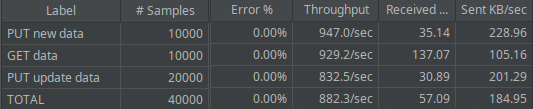
\includegraphics[width=1\textwidth]{images/stress_test_rust.png}
    \caption{Резултати тестирања \textit{Rust} сервера}
    \label{fig:stress_rust}
\end{figure}

\begin{figure}[H]
    \centering
    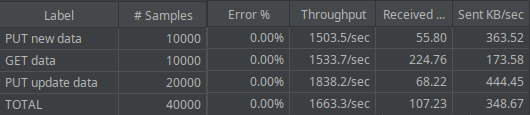
\includegraphics[width=1\textwidth]{images/stress_test_go.png}
    \caption{Резултати тестирања \textit{Go} сервера}
    \label{fig:stress_go}
\end{figure}
\pagebreak

\section{Поређење перформанси}

За мерење перформанси, услед недостатка адекватних алата, кориштен је скуп оркестрираних наменских скрипти и алата. За мерење заузећа меморије и процесора кориштен je \textit{pidstat CLI} алат \cite{pidstat}, док је за остале параметре кориштен \textit{Apache Benchmark} \cite{ab}. Тестирање започиње покретањем сервера и добављањем идентификатора његовог процеса који се затим прослеђује двема инстанцама \textit{pidstat}-a (једна за процесор друга за меморију). Затим се покреће \textit{Apache Benchmark} и након завршетка његовог рада, сви програми се гасе и своје податке чувају у одређеним фајловима. Наменска \textit{Go} скрипта затим учитава све генерисане фајлове, парсира битне податке и уписује их у једну линију \textit{CSV} фајла. Наведени кораци описани су унутар \textit{SHELL} скрипте која као улазне параметре прима величину \textit{threadpool}-a, број захтева и број паралелних конекција. Да би се максимално аутоматизовао процес, ова скрипта се позива више пута са различитим параметрима унутар још једне \textit{SHELL} скрипте. Добијени резултати агрегирани су и приказани у табелама \ref{tab:get_perf_comp} и \ref{tab:put_perf_comp}, где су називи колона, због недостатка простора, редуковани, али у тексту испод налази се легенда за њихово тумачење. Све горе наведене скрипте као и оригинални агрегирани подаци могу се пронаћи на путањи \url{https://github.com/stojanovic00/rust-go-server-comp/tree/main/profiling/shell_profiling}.

\begin{itemize}
    \item lang - language
\item psz - pool size
\item reqs - requests
\item conns - connections
\item avgcpu - avg cpu[\%]
\item maxcpu - max cpu[\%]
\item avgmem - avg mem[\%]
\item maxmem - max mem[\%]
\item ttltstt - total test time[s]
\item preqmt - per request mean time[ms]
\item trrc - transfer rate rcvd[kB/s]
\item trs - transfer rate sent[kB/s]
\item connlat - connection latency[ms]
\item connproc - connection processing time[ms]
\end{itemize}\\

\begin{sidewaystable}
  \centering
  \csvautotabular{data/get.csv}
  \caption{Поређење перформанси \textit{GET} захтева}
  \label{tab:get_perf_comp}
\end{sidewaystable}

\begin{sidewaystable}
  \centering
  \csvautotabular{data/put.csv}
  \caption{Поређење перформанси \textit{PUT} захтева}
  \label{tab:put_perf_comp}
\end{sidewaystable}

\pagebreak
На основу добијених података можемо донети одређене закључке:
\begin{itemize}
    \item Повећањем величине \textit{threadpool}-a у обе имплементације долази до повећања искориштених ресурса процесора.
    
    \item \textit{Rust} користи убедљиво мање ресурса процесора, све док величина \textit{threadpool}-a не премаши број системских нити, где тада вођство преузима \textit{Go}. Ова појава може се приписати томе да \textit{Rust} користи системске нити, док \textit{Go} користи зелене нити за покретање својих го рутина. 

    \item За фиксну величину \textit{threadpool}-a, повећањем броја паралелних конекција у обе имплементације долази до смањења искориштених ресурса процесора.

    \item Повећањем величине \textit{threadpool}-a у обе имплементације долази до повећања искориштених  меморијских ресурса, с тиме да је релативно повећање меморије драстичније у \textit{Rust} имплементацији.

    \item \textit{Rust} у свакој ситуацији користи знатно мање меморијских ресурса.

    \item \textit{Rust} имплементација у сваком случају има брже просечно време одговора на захтев.
    
    \item \textit{Rust} имплементација готово увек има већи \textit{transfer rate}, како слања тако и примања података

    \item Преласком на 1000 паралелних конекција знатно се повећава латенцијa и смањује брзина обраде конекције, где \textit{Go} има нижу латенцију, али и мању брзину обраде конекције.

    \item Као што је и очекивано, \textit{PUT} захтев захтева више ресурса за његову обраду.
    
    
\end{itemize}

\pagebreak


\section{Закључак}
У закључку овог истраживања различитих аспеката конкурентног програмирања у програмским језицима Go и Rust на примеру вишенитног сервера, могу се извести одрђени закључци.\\

Oба програмска језика нуде подршку за конкурентно програмирање, али се различито сналазе у различитим аспектима овог домена. \textit{Go} се истиче по лакшем имплементирању и употреби \textit{threadpool-а} и боље се сналази у случају повећања његове величине. С друге стране, \textit{Rust} пружа интуитивније и безбедније механизме за имплементацију конкурентног приступа складишту података, чиме се смањује ризик од грешака приликом рада са дељеним подацима.\\

Када је у питању учинак, резултати су комплексни и зависе од конкретних захтева апликације. \textit{Go} се показује као бољи избор у ситуацијама када је потребно повећати величину threadpool-a и задржати заузеће процесорске моћи у дозвољеним границама, док га \textit{Rust} у свим осталим аспектима надмашује. Овим се може закључити да мало изазовнији начин програмирања у \textit{Rust}-у, иако некада главоболан, на самом крају награђује завидним перформансама.
\pagebreak




\bibliographystyle{plain}
\typeout{}
\bibliography{biblist}              % ТОДО попуњавати референцама

\end{document}